\subsection{Observer (\textit{o Dependents, Publish-Subscribe})}
\label{observer}

\textbf{Scopo}: Comportamentale \\
\textbf{Raggio d'azione}: Oggetti

\paragraph{Definizione} Il pattern Observer permette di definire una dipendenza uno a molti tra oggetti, in modo tale che se un oggetto cambia il suo stato, tutti gli oggetti dipendenti da questo siano notificati e aggiornati automaticamente.

\paragraph{Motivazione} Un effetto collaterale comune del partizionare un sistema in una collezione di classi cooperanti è la necessità di mantenere consistenza tra oggetti correlati, ma non vuoi raggiungere la consistenza rendendo le classi strettamente accoppiate, perché questo riduce la loro riusabilità. Per esempio, molti toolkit per interfacce utente grafiche separano gli aspetti di presentazione dell'interfaccia utente dai dati applicativi sottostanti, dove le classi che definiscono dati applicativi e presentazioni possono essere riutilizzate indipendentemente e possono anche lavorare insieme: sia un oggetto foglio di calcolo che un oggetto grafico a barre possono rappresentare informazioni nello stesso oggetto dati applicativi usando diverse presentazioni, dove il foglio di calcolo e il grafico a barre non si conoscono reciprocamente, permettendoti così di riutilizzare solo quello di cui hai bisogno, ma si comportano come se si conoscessero. Quando l'utente cambia le informazioni nel foglio di calcolo, il grafico a barre riflette i cambiamenti immediatamente, e viceversa, e questo comportamento implica che il foglio di calcolo e il grafico a barre dipendono dall'oggetto dati e quindi dovrebbero essere notificati di qualsiasi cambiamento nel suo stato, senza ragioni per limitare il numero di oggetti dipendenti a due poiché ci può essere qualsiasi numero di diverse interfacce utente per gli stessi dati.

\begin{figure}[H]
    \centering
    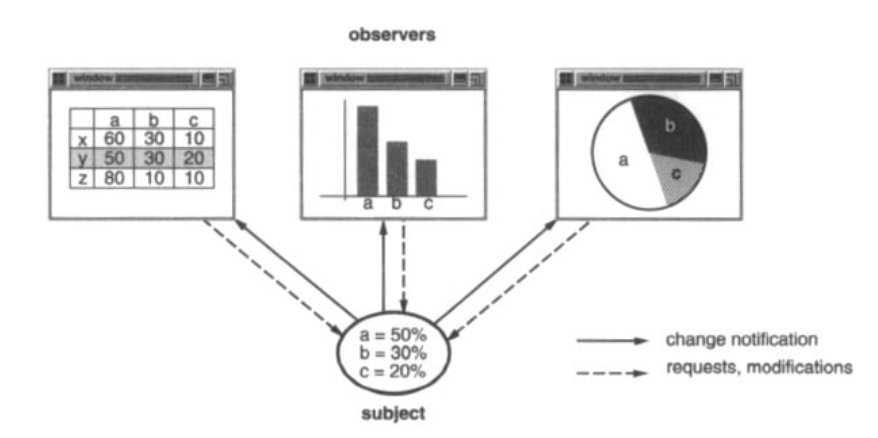
\includegraphics[width=0.5\linewidth]{assets/pattern/observer/observer-esempio.png}
\end{figure}

Il pattern Observer descrive come stabilire queste relazioni, dove gli oggetti chiave sono subject e observer: un subject può avere qualsiasi numero di observer dipendenti, tutti gli observer vengono notificati ogni volta che il subject subisce un cambiamento di stato, e in risposta ogni observer interrogherà il subject per sincronizzare il suo stato con quello del subject. Questo tipo di interazione è anche conosciuta come publish-subscribe, dove il subject è il publisher delle notifiche che invia senza dover sapere chi sono i suoi observer, e qualsiasi numero di observer può sottoscriversi per ricevere notifiche.

\newpage

\paragraph{Applicabilità} È opportuno usare il pattern Observer quando:
\begin{itemize}
    \item Un'astrazione ha due aspetti, uno dipendente dall'altro. Incapsulare questi aspetti in oggetti separati consente di variarli e riutilizzarli in modo indipendente.
    \item Una modifica a un oggetto richiede la modifica di altri oggetti e non si sa quanti oggetti devono essere modificati.
    \item Un oggetto deve essere in grado di notificare altri oggetti senza fare supposizioni su chi siano questi oggetti. In altre parole, non si desidera che questi oggetti siano strettamente accoppiati.
\end{itemize}

\begin{figure}[H]
    \centering
    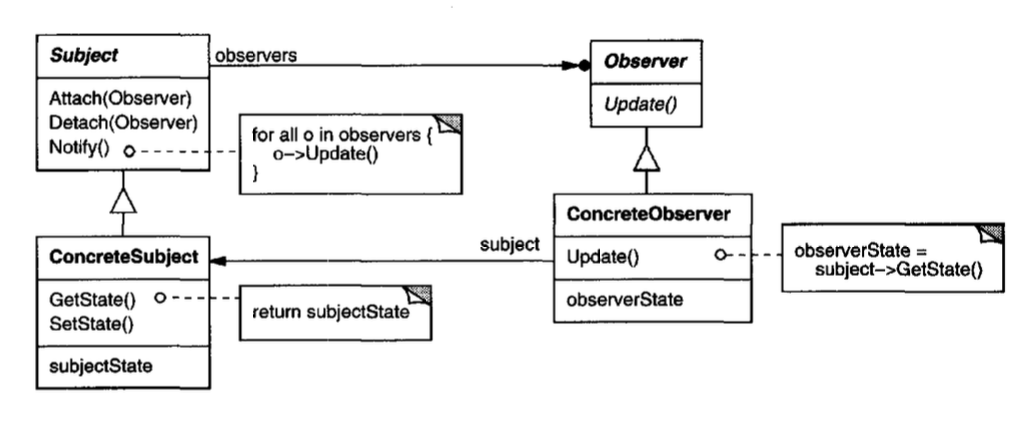
\includegraphics[width=0.75\linewidth]{assets/pattern/observer/observer-struttura.png}
    \caption{Class Diagram del pattern Observer}
\end{figure}

\paragraph{Struttura} Il pattern è composto da:
\begin{itemize}
    \item \textbf{Subject}: conosce i propri osservatori; un numero qualunque di oggetti Observer può osservare un soggetto. Fornisce un’interfaccia per registrare e cancellare le registrazioni degli oggetti Observer.
    \item \textbf{Observer}: fornisce un’interfaccia di notifica per gli oggetti a cui devono essere notificati i cambiamenti nel Subject.
    \item \textbf{ConcreteSubject}: contiene lo stato a cui gli oggetti ConcreteObserver sono interessati. Inoltra una notifica ai suoi Observer quando il proprio stato si modifica.
    \item \textbf{ConcreteObserver}: memorizza un riferimento a un oggetto ConcreteSubject oppure ottiene dinamicamente il riferimento all’oggetto Subject da cui ha origine la notifica in caso in esso cui osservi più Subject. Contiene informazioni che devono essere sincronizzate con lo/gli stato/i del/i Subject. Implementa l’interfaccia Observer per ricevere le notifiche del Subject.
\end{itemize}


\begin{figure}[H]
    \centering
    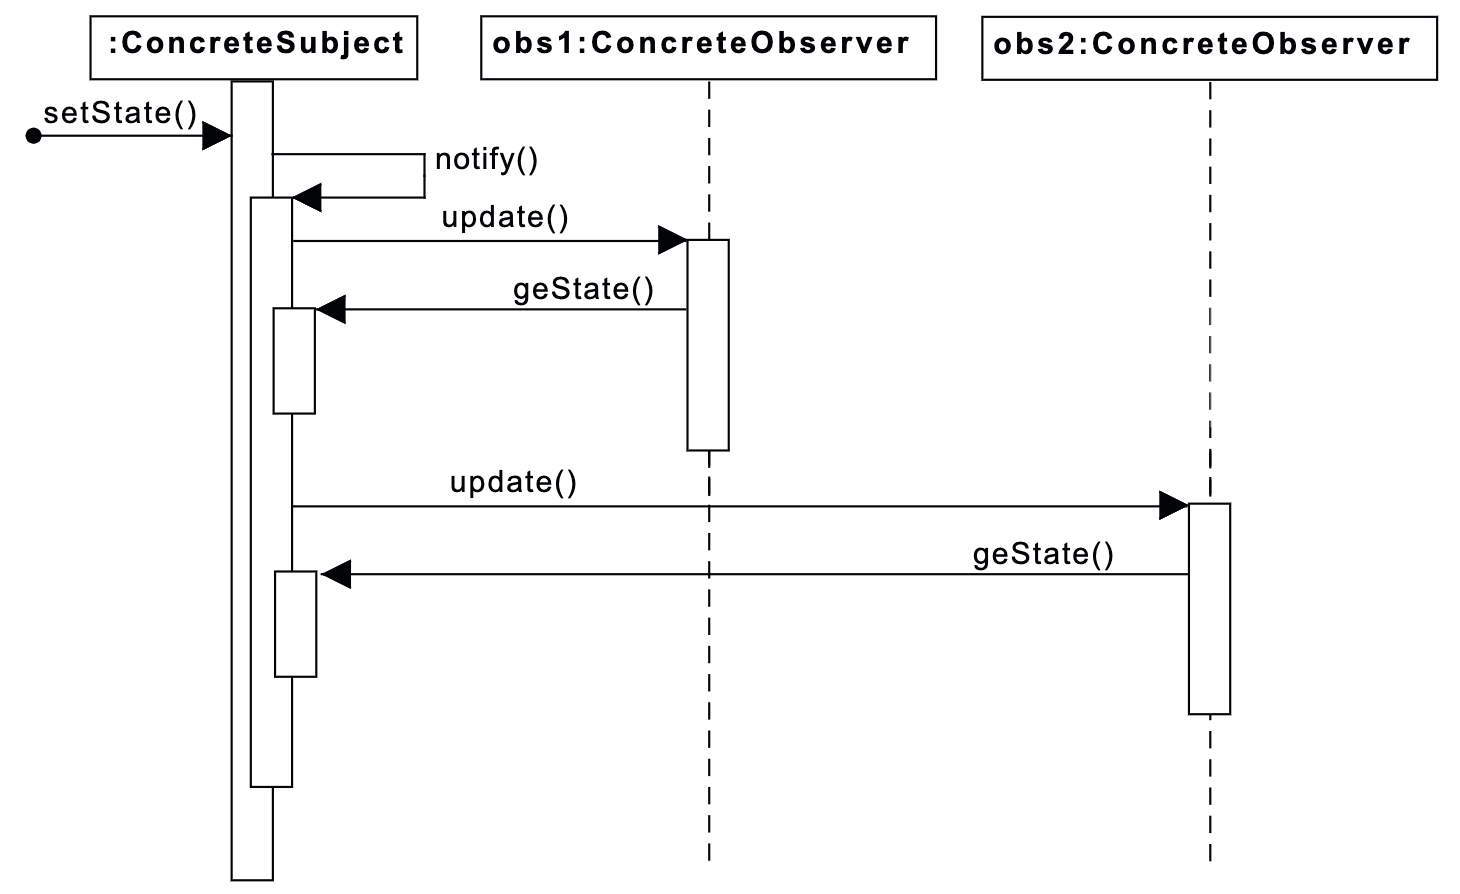
\includegraphics[width=0.75\linewidth]{assets/pattern/observer/observer-sequence.png}
    \caption{Sequence Diagram del pattern Observer}
\end{figure}

ConcreteSubject notifica i propri Observer quando avviene un cambiamento che potrebbe rendere il loro stato non inconsistente rispetto al proprio. Dopo essere stato informato di un cambiamento nel ConcreteSubject, un ConcreteObserver può chiedere al Subject informazioni sul suo stato. ConcreteObserver usa questa informazione per riconciliare il suo stato con quello del subject.

\paragraph{Conseguenze} Il pattern Observer consente quindi di:
\begin{itemize}
    \item Avere un accoppiamento astratto tra Subject e Observer.
    \item Supportare la comunicazione broadcast.
\end{itemize}

È bene notare che, in base a come viene implementato, il pattern potrebbe provocare degli aggiornamenti imprevisti.

\newpage